\documentclass[10pt]{beamer}
\setbeamertemplate{navigation symbols}{\insertlogo}

%\documentclass[handout,dvips,11pt,grey]{beamer}

%\usetheme{Goettingen}
%\usetheme{Warsaw}
\usetheme{Hannover}

%\usepackage{tikz,pgf}
\usepackage{xcolor}
\usepackage{multicol}
\usepackage{amsmath,amsthm,amssymb}
%\usepackage{epstopdf}
\usepackage{xspace}
\usepackage{wrapfig}

\usepackage{verbatim}
%\usepackage{circuitikz}
%\usepackage{graphicx}
\usepackage{comment}
%\usepackage{array}
\usepackage{coffee4}


\title{Understanding and Using Topic Modeling}
\subtitle{Using inferred document clusters}
\author{Philip Robinson}
\date{\today}
\institute{Presented to Knowlege Mavens}

\DeclareMathOperator*{\argsort}{argsort}

  \logo{
\includegraphics[height=.7cm]{./logo.png}}

\begin{document}

\begin{frame}
  \titlepage

\end{frame}


\begin{frame}{Presentation Overview}
  \tableofcontents

\end{frame}

\section{What is Topic Modeling}

\begin{frame}{What is Topic Modeling}
  {\bf Our goal: mathematically model topics from a corpus}

  \begin{quote}
    Topic modeling is a text processing technique for automatically grouping documents by topics. This is usually used as a strategy to describe documents in low dimensional space or an exploratory tool for document collections.
  \end{quote}
\end{frame}

\newcommand{\Food}[1]{\colorbox{orange!30}{#1}\xspace}
\newcommand{\Travel}[1]{\colorbox{blue!30}{#1}\xspace}
\newcommand{\Time}[1]{\colorbox{green!30}{#1}\xspace}
\newcommand{\Document}[1]{\fbox{\begin{minipage}{\columnwidth}#1\end{minipage}}}



\begin{frame}{Examples}
{\bf In practice, this requires many more documents}

  \begin{multicols}{2}

    \Document{
      The \Travel{Tourist} huddles in the \\ \Travel{station} While slowly \Time{night} gives way to \Time{dawn}; He finds a certain fascination In knowing all the \Travel{trains} are gone.
    }

    \vspace{.25em}

    \Document{
      The Governess up in the attic \\Attempts to make a cup of \Food{tea}; Her mind grows \Time{daily} more erratic From cold and \Food{hunger} and ennui.
    }

    \vspace{.25em}

    \Document{
      The Journalist surveys the slaughter, The best in \Time{years} without a doubt; He pours himself a \Food{gin} and \Food{water} and wonders how it came about.
    }

    \columnbreak

    \begin{itemize}
    \item \Food{Food}
    \item \Travel{Travel}
    \item \Time{Time}
    \end{itemize}

    \vspace{1em}

    From this annotation we know that Document 2 and 3 are about \Food{Food} and \Time{Time}
  \end{multicols}

\end{frame}

\section{Why Topic Model}
\begin{frame}{What can I solve?}
  \begin{itemize}
  \item Find similar document pairs
  \item Cluster documents into groups with similar content
  \item Find relevant documents to a query or user's interests
  \item Explore shape of document collection
  \end{itemize}

  \begin{quote}
    Topic modeling can usually be extended to address many other problems, and document embeddings can be used to inform downstream models.
  \end{quote}
\end{frame}

\begin{frame}{Applications of Topic Modeling}

  \begin{multicols}{4}

  \begin{figure}
  \includegraphics[width=\columnwidth]{full2.png}

  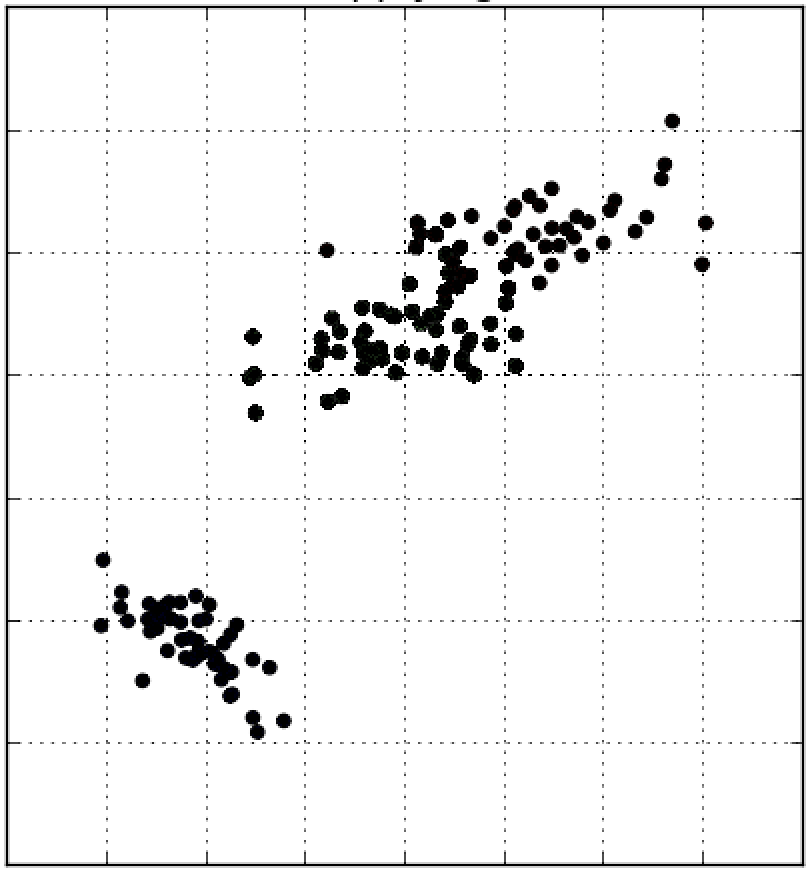
\includegraphics[width=.8\columnwidth]{reduced.png}
  \caption{Dimmentionality Reduction}
  \end{figure}
  \columnbreak

  \hfill
    \begin{figure}
  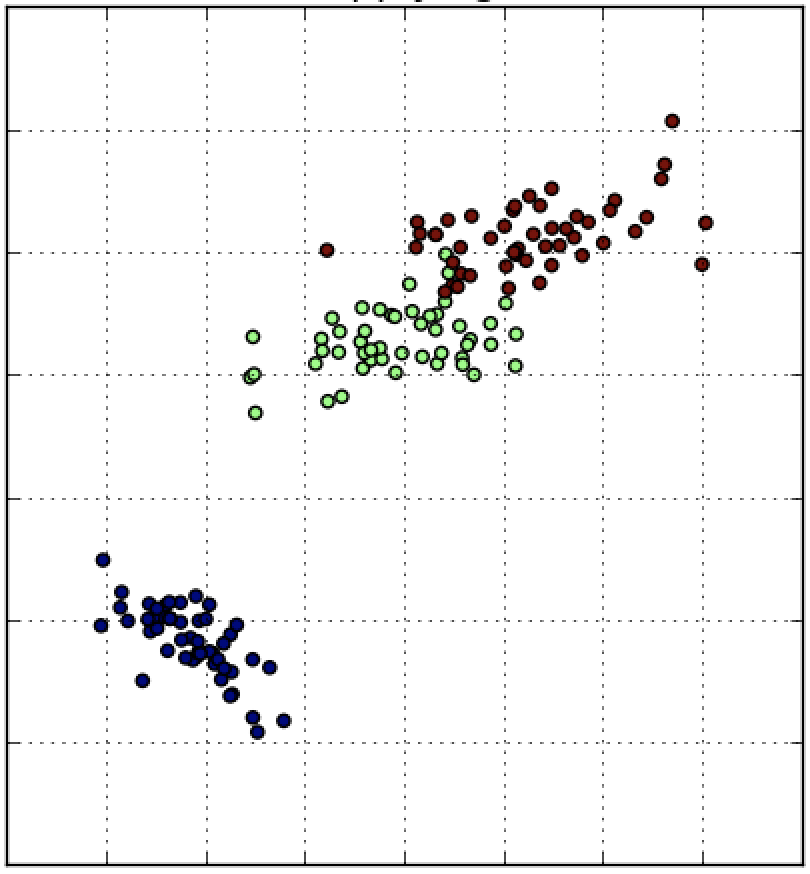
\includegraphics[width=\columnwidth]{cluster.png}
  \caption{Cluster Points}
  \end{figure}
    \columnbreak

  \hfill
    \begin{figure}
  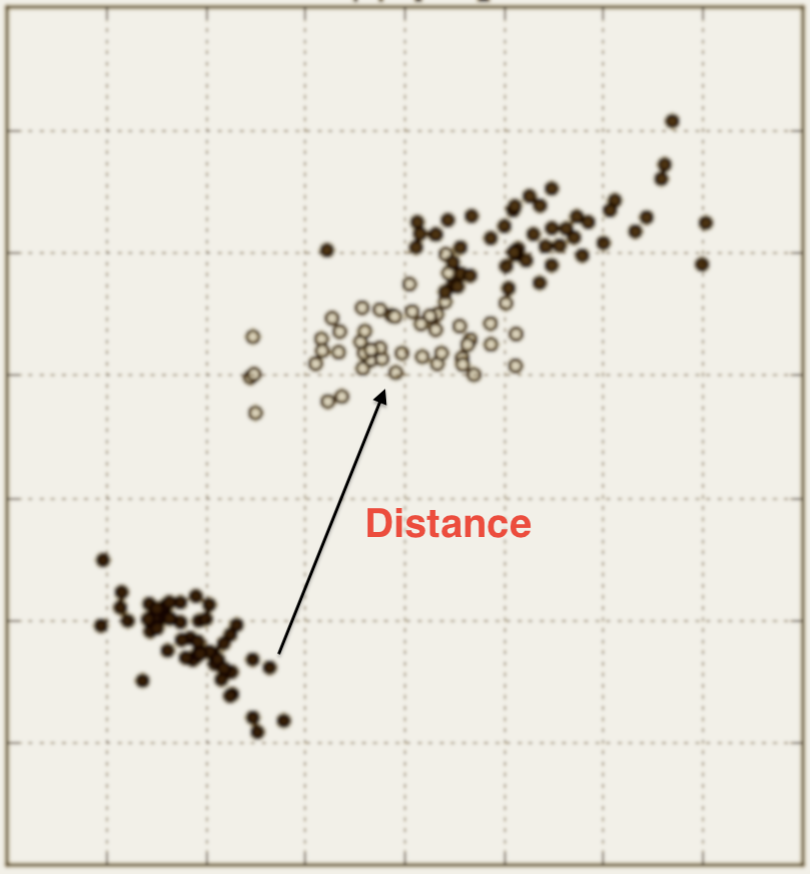
\includegraphics[width=\columnwidth]{dist.png}
  \caption{Exploratory Data Analysis}
  \end{figure}
    \columnbreak

  \hfill
    \begin{figure}
  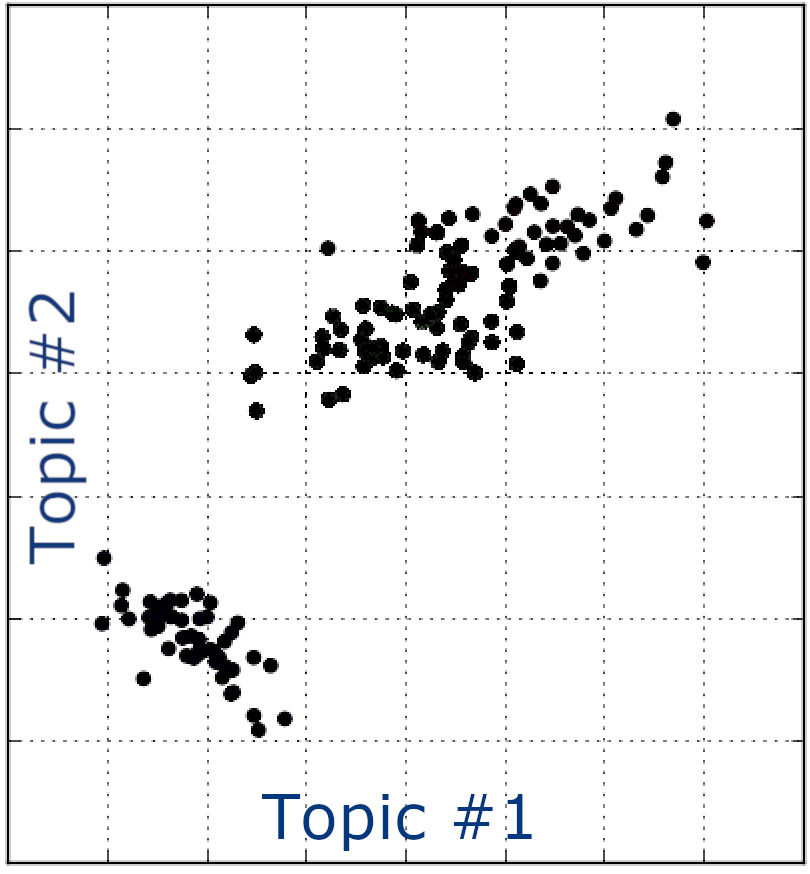
\includegraphics[width=\columnwidth]{topicanalysis.png}

  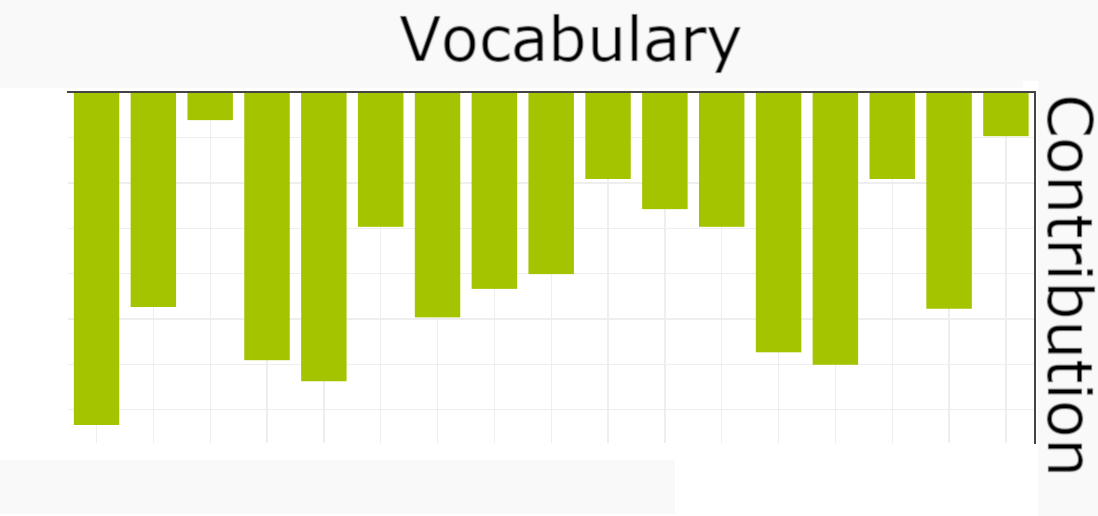
\includegraphics[width=\columnwidth]{bar-simple.png}
  \caption{Analysis of Topics}
  \end{figure}

  \end{multicols}

\end{frame}


\section{Generative Models}
\begin{frame}{Goals of generative models}
  {\bf A generative model}

  \begin{itemize}
  \item Assume/Generalize how data could have been generated
  \item Fit distributions that describe the generalization
  \item Ask questions about the generalization in relation to data
  \item Ask questions about data in relation to the generalization
  \end{itemize}

  \vspace{1em}

  \begin{quote}
    Generative models are much easier to extend, because they abstract the model from it's linear algebra dependencies.

    \vspace{1em}

  Topic modeling generalizes how a document is generated by claiming that words come from topics, and documents have multiple topics.\footnote{this is not a language model} %Note that this ignores sentence structure, entities, authorship, or other things we may care about.

  \end{quote}

\end{frame}

\begin{frame}{Latend Dirichlet Allocation}
  {\bf Bayesian extension to PLSA}

  \begin{multicols}{2}

  \begin{itemize}
  \item Represent document as Bag-of-Words\footnote{equivalent to multinomial over the vocabulary}
  \item Model/Fit topics as mixture of words
  \item Documents are projected into or sampled from topic-space-distribution
  \end{itemize}

  \begin{figure}
  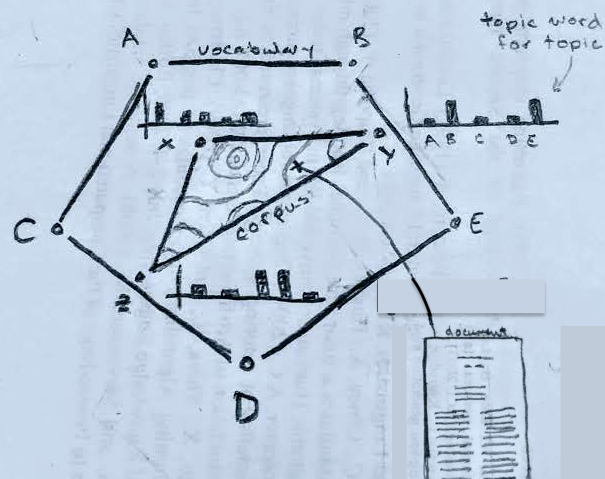
\includegraphics[width=\columnwidth]{./lda-draw.png}
  \caption{Latent Dirichlet Allocation}
  \end{figure}

  \end{multicols}

  \begin{quote}
    Enormous body of work extending this model to address more specific problems.
  \end{quote}

\end{frame}

\section{Understanding Model Space}

\begin{frame}{Looking at top words}
  {\bf Mitigating apophenia is hard, topics difficult to interpret}

  \begin{multicols}{3}
    Topic \#1
    \begin{itemize}
    \item server
    \item connected
    \item access
    \item workstation
    \item outage
    \item user
    %\item service
    %\item restart
    \end{itemize}

    \columnbreak

    Topic \#2
    \begin{itemize}
    \item mode
    \item instrument
    \item safe
    \item spacecraft
    \item anomaly
    \item recovery
    %\item event
    %\item control
    \end{itemize}

    \columnbreak

    Topic \#3
    \begin{itemize}
    \item uplink
    \item station
    \item dsn
    \item spacecraft
    \item lock
    \item ace
    %\item bps
    %\item radiation
    \end{itemize}

  \end{multicols}

  \begin{quote}
    Although the model better describes our generation process, from the perspective of topics, it can be difficult to know what these topics actually represent.\footnote{Supervised LDA attempts to addresses this\\ concern, also applies to sentiment analysis} This may require experts who are immune to apophenia.
  \end{quote}
\end{frame}


\begin{comment}
\begin{frame}{Evaluation}
  {\bf Does our fit dirichlet distribution describe our data or our understanding}

  \begin{itemize}
  \item perplexity
  \item coherence
  \item visualization
  \item predictive power
  \end{itemize}
\end{frame}

\begin{frame}{Perplexity vs Coherence}
  {\bf perplexity for prediction, coherence for EDA\footnote{exploratory data analysis}}

  \begin{quote}
    Perplexity measures how poorly the model describes the data.
  \end{quote}

  \begin{align*}
    Perplexity(q) &= b^{-\frac{1}{N}\sum_{x \in X} log_b q(x)}
  \end{align*}

  \begin{quote}
    Topic coherence measures take the set of $N$ top words from a topic and sums a \texttt{confirmation measure}\footnote{like pointwize mutual information (PMI)} over the word pairs. Probabilities are estimated from sliding window over train and test corpora.
  \end{quote}

  \begin{align*}
    C_{Irvine} &= \frac{2}{N\cdot N-1}\sum_{i=1}^{N-1}\sum_{j=i+1}^N PMI(w_i, w_j)\\
    PMI(w_i, w_j) &= log(\frac{P(w_i, w_j)}{P(w_i)\cdot P(w_j)})
  \end{align*}
\end{frame}

\begin{frame}{Interactive Visualization\footnote{used \texttt{pyLDAvis}}}
  {\bf Breakout to jupyter}

    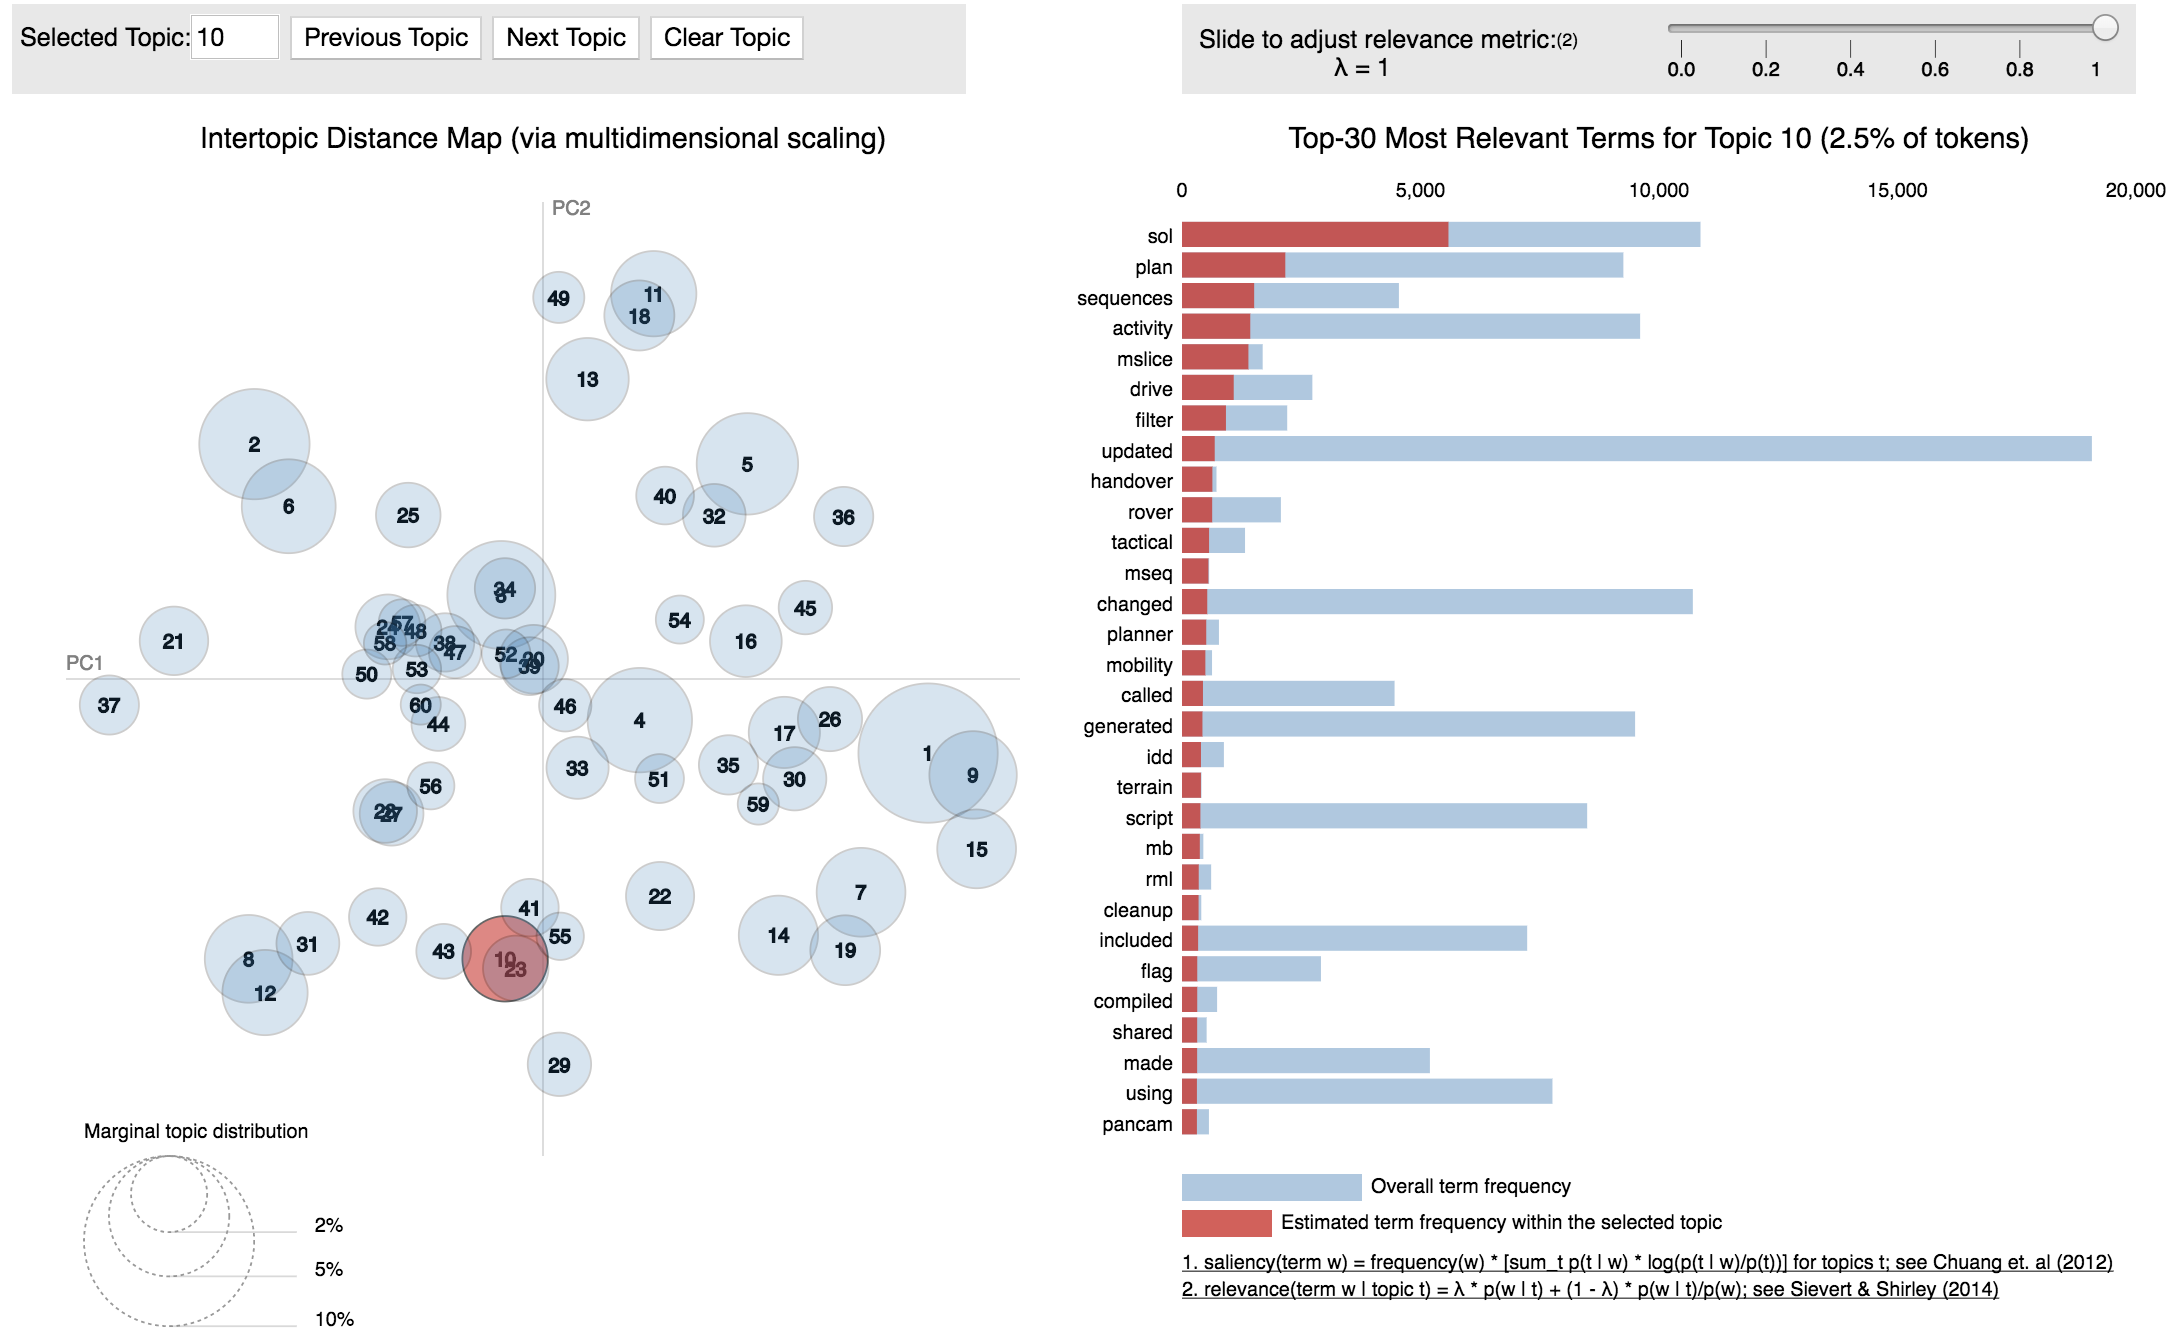
\includegraphics[width=\textwidth]{LDAvis.png}

\end{frame}
\end{comment}

\section{After LDA}
\begin{frame}{Extensions}
  \begin{itemize}
  \item Entity Boosted Topic Model (ETM)
  \item[$\rightarrow$] Author Topic Model (ATM)
  \item Hierarchical Dirichlet Process (HDP)
  \end{itemize}
\end{frame}

\end{document}
